%!TEX root = ../../Thesis.tex

\section{Evaluation: OLTP Workloads}
\label{sec:oltp}

OLTPBench \cite{DBLP:journals/pvldb/DifallahPCC13} is a benchmark suite of representative 
OLTP workloads for relational databases.
%, obtained from applications such as
%wholesale supply, banking, seat booking, voting, collaborative-editing and so on. 
%OLTPBench consists of a configurable 
%load generator that takes care of populating database tables, followed by
%issuing various different transactions in a desired proportion. 
We picked a subset of OLTPBench for which we had reasonable assertions. 
Table~\ref{table-bench} lists basic
information such as the number of database tables, the
number of static transactions, how many of them are read-only, and the number of
different assertions corresponding to system invariants for testing the benchmark. 
%We included TPC-C, the
%most widely known benchmark, and a few others for which we could come up with
%reasonable assertions. 
We modified OLTPBench by rewriting SQL join and aggregation
operators 
%(16.67\% of total queries) 
into equivalent application-level
loops, following a similar strategy as prior work \cite{DBLP:journals/pacmpl/RahmaniNDJ19}. Except for
this change, we ran OLTPBench unmodified. 

For TPC-C, we obtained a set of $12$ invariants from its specification
document~\cite{tpcc-spec}. For all other benchmarks, we manually identified 
invariants that the application should satisfy. We asserted these invariants 
by issuing a read-only transaction to \tool{} 
at the end of the execution of the benchmark. 
None of the assertions fail under serializability; they are indeed invariants
under serializability.\footnote{We initially observed two assertions failing
under serializability. Upon analyzing the code, we identified that the
behavior is due to a bug in OLTPBench that we have reported to the authors (link
ommitted).} 
%We use \tool{} to test their
%validity under causal consistency and read committed isolation levels. 
When using weaker isolation, we configured MonkeyDB to use latest reads only
(\sectref{impl}) for the assertion-checking transactions 
in order to isolate the weak behavior to only the application. 

We ran each benchmark $100$ times and report, for each assertion, the number of
runs in which it was violated. Note that OLTPBench runs in two phases. The first
is a loading phase that consists of a big initial transaction to populates tables 
with data, and then the execution phase issues multiple concurrent transactions. 
With the goal of testing correctness, we \textit{turn down} the scale factor to
generate a small load and limit the execution phase time to ten seconds with 
just two or three sessions. A smaller test setup has the advantage
of making debugging easier. With \tool{}, there is no need to generate large
workloads.

%We first discuss our results on TPC-C~\cite{tpcc-bench} in detail followed by
%other benchmarks,
% as TPC-C specifies its invariants and all its invariants are well studied by
% previous works~\cite{DBLP:journals/pacmpl/RahmaniNDJ19,DBLP:journals/pvldb/GanRRB020}.
%We first discuss our results on SmallBank, SEATS, Voter and Wikipedia, followed by TPC-C in detail.

\begin{table}
  \centering
  \footnotesize
	\begin{tabular}{|l|c|c|c|c|}
    \hline
		Benchmark & \#Tables & \#Txns &\#Read-only & \#Assertions \\ \hline
		TPC-C &  9 & 5 & 2& 12\\
		SmallBank & 3 & 6 & 1 & 1\\
		Voter & 3 & 1 & 0 & 1\\
		Wikipedia & 12 & 5 & 2 & 3\\
		\hline
	\end{tabular}	
	\caption{OLTP benchmarks tested with \tool{}}
	\label{table-bench}
\end{table}


\paragraph{TPC-C} TPC-C emulates a wholesale supplier transactional system
that delivers orders for a warehouse company.
This benchmark deals with customers, payments, orders, warehouses, 
deliveries, etc. 
%As listed in Table~\ref{table-bench}, it has five transactional procedures, out
%of which three (new order, payment and delivery) modify the database and two
%(order status and stock level) are read-only.
We configured OLTPBench to issue a higher proportion ($>85\%$) of update
transactions, compared to read-only ones.  
%(29, 29, 8, 29, 5)
Further, we considered a small input workload constituting of one warehouse, two
districts per warehouse and three customers per district.

%TODO A12 IS THE ASSERTION WHERE WE REPLACED EQUALITY WITH >= ?
%Ans: NO. THAT IS A11

TPC-C has twelve assertions (A1 to A12) that check for consistency between 
the database tables.
For example, A12 checks: for any customer, the sum of delivered order-line
amounts must be equal to the sum of balance amount and YTD (Year-To-Date)
payment amount of that customer.
%C_BALANCE + C_YTD_PAYMENT = sum(OL_AMOUNT)
%We observed that all these assertions succeed under Serializability, 
%when tested both on \tool{} and on a real database
%MariaDB~\cite{mariadb}\footnote{We initially observed two assertions failing
%under Serializability. Upon analyzing the code, we identified that the
%behavior is due to a bug in OLTPBench that we have reported to the authors (link
%ommitted).}. 
%(\url{https://github.com/oltpbenchmark/oltpbench/issues/345}).}.
%We ran TPC-C for 100 times.
%To test whether they preserve under weak behaviors, we run the benchmark on
%\tool{} under Causal and Read Committed isolation levels, for 100 test
%iterations.

\begin{figure*}[!ht]
    \centering
    \begin{minipage}{\textwidth}
        \centering
    	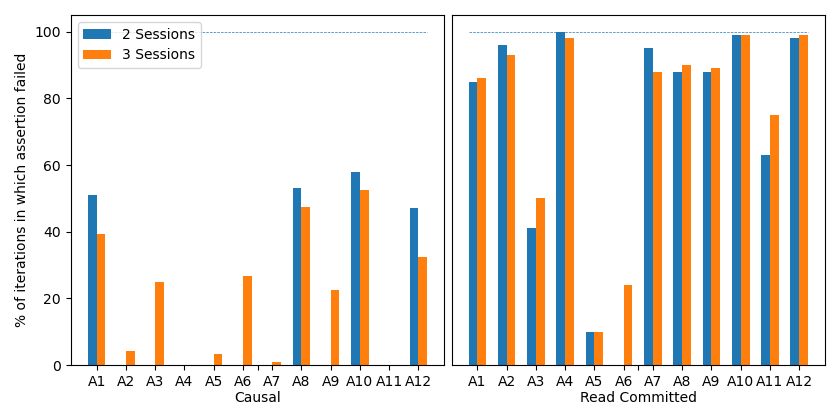
\includegraphics[scale=0.4]{Sources/sql/plots/random_strongest_tpcc.png}
	    \caption{Assertion checking: {TPC-C}}
        \label{fig:tpcc}
	\end{minipage}
	
    \begin{minipage}{\textwidth}
        \centering
		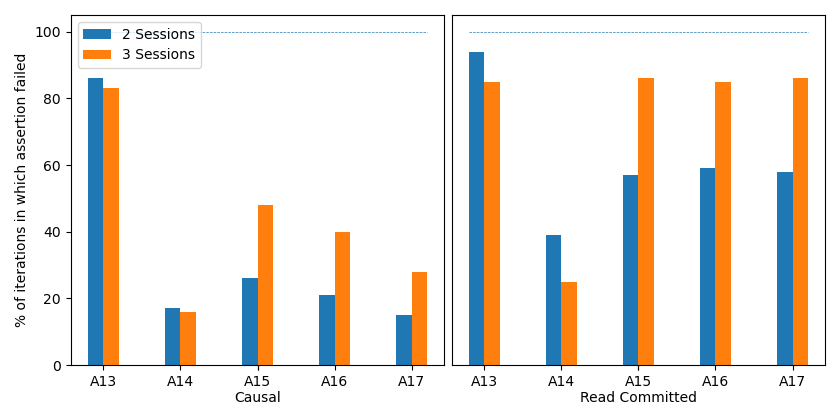
\includegraphics[scale=0.4]{Sources/sql/plots/random_strongest_all.png}
	    \caption{Assertion checking: SmallBank, Voter, and Wikipedia}
    \label{fig:rest}
    \end{minipage}
\end{figure*}

Figure~\ref{fig:tpcc} %and Figure~\ref{fig:tpcc-rc} 
shows the percentage of test runs in which an assertion failed. 
%Figure~\ref{fig:tpcc-rc} 
It shows that all the twelve assertions are violated under
Read~Committed isolation level. In fact, $9$ out of the $12$ 
assertions are violated in more than 60\% of the test runs.
In case of causal, %(Figure~\ref{fig:tpcc}), 
all assertions are violated
with three sessions, except for A4 and A11. We manually inspected TPC-C and
we believe that both these assertions are valid under causal consistency. 
For instance, A4 checks for consistency between two tables, both of which are
only updated within the same transaction, thus causal consistency is enough to
preserve consistency between them.
%For instance, A04 checks that for each district, the number of order lines of all 
%the orders in that district (obtained from ORDER\_LINE table) is the same as 
%the sum of order-line counts maintained for the corresponding orders (in the ORDER
%table). Both the concerned tables (ORDER\_LINE and ORDER) are updated within the same transaction,
%thus causal consistency is enough to ensure that they remain consistent with each
%other. 

%These results demonstrate the effectiveness of \tool{} in breaking (invalid) 
%assertions.

%To understand why A04 and A11 did not violate under Causal, we analyzed the two
%assertions and the transactional procedures associated with them in TPC-C.
%In our analysis, we found that it is not possible to violate A04 and A11 under
%Causal or any other stronger isolation levels.
%For example, A04 checks for every district, the number of order lines of all 
%the orders in that district (obtained from ORDER\_LINE table) is same as 
%the sum of order-line counts maintained for the corresponding orders (in ORDER
%table).
%This assertion cannot be violated under Causal because the insertions to both
%tables happen atomically in a single transactional procedure (`new
%order').
%A04: For every district, the number of orderlines of all orders is same as sum of orderline count (number of orderlines). %defined in order table.  
%sum(O_OL_CNT) = [number of rows in the ORDER-LINE table for this district]
%A11: For every district and every customer, the difference between number of orders and number of new orders must be equal to 2100.
%(count(*) from ORDER) - (count(*) from NEW-ORDER) = 2100

%\akash{This para can be skipped.}
%We also observed that MonkeyDB's read selection strategy had minor impact on the
%results. Choosing weakest-read gave geo-mean disimprovement of 27.1\%,
%whereas weak-biased-read gave geo-mean disimprovement of 61.7\%.   
%Similarly, instead of strongest-read strategy for the assertion checks, we
%used the same read strategy as the one used for the test. In this case, 
%random-read gave a geo-mean disimprovement of 36.2\%, weakest-read gave 
%geo-mean disimprovement of 53.9\%, weak-biased-read gave a geo-mean
%disimprovement of 73.7\%.
%These numbers indicate that the default random-read and strongest-read strategy
%combination works well in practice.

These results demonstrate the effectiveness of \tool{} in breaking (invalid) 
assertions. Running with MySQL, under read committed, was unable to violate any assertion except for
two (A10 and A12), even when increasing the number of sessions to $10$. We used
the same time limit of $10$ seconds for the execution phase. We note that MySQL
is much faster than MonkeyDB and ends up processing up to $50\times$ more
transactions in the same time limit, yet is unable to violate most assertions. 
Prior work \cite{DBLP:journals/pacmpl/RahmaniNDJ19} attempted a more sophisticated test
setup where TPC-C was executed on a Cassandra cluster, while running 
Jepsen~\cite{jepsen} for fault injection. This setup also was unable to violate 
all assertions, even when running without transactions, and on a weaker isolation level than read committed. 
Only six assertions were violated with 10 sessions, 
eight assertions with 50 sessions, and ten assertions with 100 sessions.
With \tool{}, there is no need to set up a cluster, use fault injection or
generate large workloads that can make debugging very difficult. 


%\begin{figure}
%    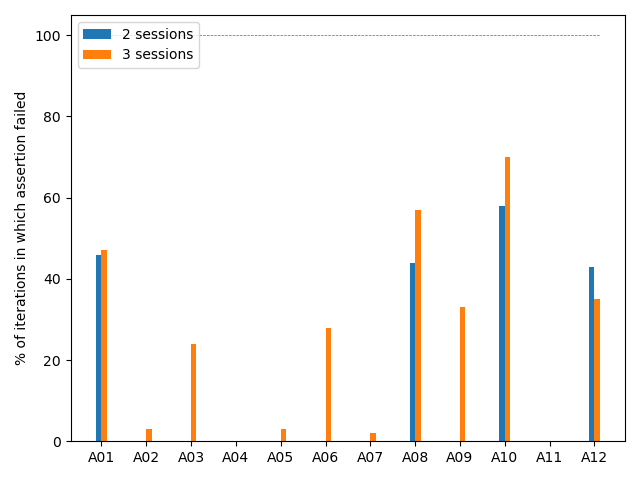
\includegraphics[scale=0.4,width=0.48\textwidth]{plots/tpcc_causal.png}
%    \caption{Assertion Violations under Causal Consistency.}
%    \label{fig:tpcc-causal}
%\end{figure}
%\begin{figure}
%    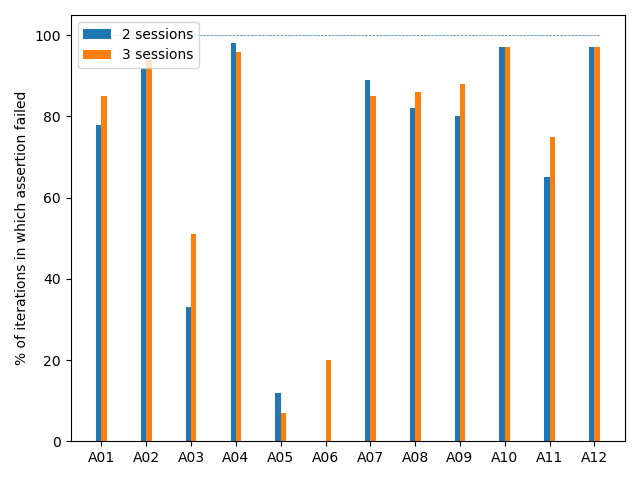
\includegraphics[scale=0.4,width=0.48\textwidth]{plots/tpcc_readcommitted.png}
%    \caption{Assertion Violations under Read Committed.}
%    \label{fig:tpcc-rc}
%\end{figure}
%

\paragraph{SmallBank, Voter, and Wikipedia} 
SmallBank is a standard financial banking system, dealing with customers, saving
and checking accounts, money transfers, etc.  
Voter emulates the voting system of a television show and allows users to vote for their favorite contestants.
%Concurrent votes by a user to the same contestant brings in complexity to the voting system. 
Wikipedia is based on the popular online encyclopedia. It deals with a complex database schema involving 
page revisions, page views, user accounts, logging, etc.  
It allows users to edit its pages and maintains a history of page edits and user actions. 
%Data contention in this system arises when multiple users edit the same page or when the same user edits a page from multiple sessions.

We identified a set of five assertions, A13 to A17, that should be satisfied by these systems.  
%Among the five assertions, three are from Wikipedia, and one each from SmallBank and Voter systems.
For SmallBank, we check if the total money in the bank remains the same while it
is transfered from one account to another (A13). 
Voter requires that the number of votes by a user is limited to a fixed threshold (A14).  
For Wikipedia, we check if for a given user and for a given page, the number of
edits recorded in the user information, history, and logging tables
%(USERACCT, RECENTCHANGES, and LOGGING tables) 
are consistent (A15-A17). 
%All these assertions are preserved under Serializability isolation level.
%We test these systems on \tool{} for assertion violations under Causal and Read Committed isolation levels.
%For all these benchmarks, we configure the weights of transactional procedures in OLTP-Bench 
%such that the transactions which update are executed more often.   
As before, we consider small work loads: (1) five customers for SmallBank, (2) one user for Voter, and (3) two pages and two users for Wikipedia.  

Figure~\ref{fig:rest} shows the results. 
\tool{} detected that all the assertions are invalid under the chosen isolation levels.
Under causal, \tool{} could break an assertion in 26.7\% (geo-mean) runs given 2 sessions and in 37.2\% (geo-mean) runs given 3 sessions.
Under read committed, the corresponding numbers are 56.1\% and 65.4\% for 2 and
3 sessions, respectively.
%Our results in this experiment confirm the generality and effectiveness of \tool{} in detecting assertion violations in diverse OLTP environments. 

%\begin{figure}[t]
%    \includegraphics[scale=0.4,width=0.48\textwidth]{plots/all_random_strongest.png}
%    \caption{\small Assertions violated under Causal and Read~Committed}
%    \label{fig:diverse-bench}
%\end{figure}
